\documentclass[../Main.tex]{subfiles}
\begin{document}
\title{\textbf {Math 28B: Introduction to Rings and Fields}\\[0.2em]\large Based on Lectures by Mckee Krumpak\vspace{-2ex} }
\author{Typed by Hussein Hijazi}
\date{Spring 2021}
\titlepic{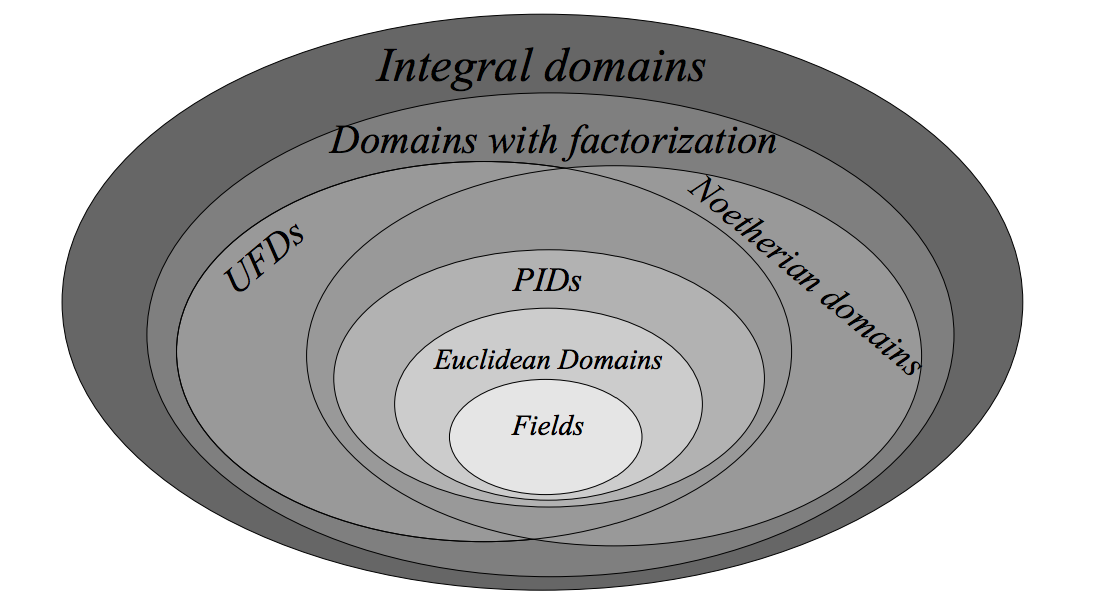
\includegraphics[width=0.85\textwidth]{rings.png}}
\begin{minipage}{\textwidth}
\maketitle
\textbf{Disclaimer:} These notes are typeset versions of the recorded lectures and are often modified with my own exposition to help clarify and understand ideas professed in the lectures. All errors in these notes are (almost surely) mine and are thus my responsibility. The permanent link to this document is found on \href{https://hushus46.github.io/28B-Notes/}{https://hushus46.github.io/28B-Notes}\\

I try my best to keep the multiplication of ring elements (with the $\rdot $ operation) explicit, but sometimes I have left it out unintentionally as the notes were typed (this happens more often in earlier lectures). The spacing of nested proofs and claims can be a bit awkward; occasionally, I will go back through the notes to make it more readable.\\

The table of contents is set up to easily navigate between presented ideas, although I haven't been able to think of titles for everything.\\ 

If there are any mathematical typos/errors or suggestions on design changes and theorem names, please do not hesitate to let me know at \href{mailto:husseinhijazi@brandeis.edu}{husseinhijazi@brandeis.edu}\\


\end{minipage}
\end{document}